% Afficher des recommendations concernant la syntaxe.
\RequirePackage[orthodox,l2tabu]{nag}
\RequirePackage{luatex85}
% Paramètres du document.
\documentclass[%
a5paper%                       Taille de page.
,11pt%                         Taille de police.
,DIV=15%                       Plus grand => des marges plus petites.
,titlepage=off%                 Faut-il une page de titre ?
%,headings=optiontoheadandtoc%  Effet des paramètres optionnels de section.
%,headings=small%
,parskip=false%
,openany%
]{scrbook}
\renewcommand*\partheademptypage{\thispagestyle{empty}}
\newcounter{facteur}\setcounter{facteur}{17}%%%%%%%%%%%%%% Paramètre pour la taille globale des partitions. par défaut~: 17
%\usepackage{geometry}
\usepackage{gredoc,mudoc,lyluatex}
\usepackage{pdfpages,transparent,array,ltablex}
\usepackage{framed}
\usepackage{wrapfig}

%%%%%%%%%%%%%%%%%%%%%%% Paramètres variables %%%%%%%%%%%%%%%%%%%%%%%%%%%%%%%%%%%%%%%%%%%%%%%%%%
%%% Taille des partitions grégoriennes.                                                      %%
%\grechangedim{overhepisemalowshift}{.7mm}{scalable} %%Distance to place a a horizontal episema over a note in a low position in the space.Default: 0.02287 cm
%\grechangedim{hepisemamiddleshift}{1.4mm}{scalable} %%Distance to place a horizontal episema in the middle of a space. Default: 0.07206 cm
%\grechangedim{overhepisemahighshift}{2.1mm}{scalable} %% Distance to place a horizontal episema over a note in a high position in the space. Default: 0.10066 cm
%\grechangedim{vepisemahighshift}{2.1mm}{scalable} %% Distance to place a vertical episema in a high position in the space. Default: 0.06634 cm
%\grechangestafflinethickness{50} %%% epaisseur des lignes The default value is same as staff size.
\grechangestaffsize{\value{facteur}}%%%%% 
%%%%%%%%%%%%%%%%%%%%%%%%%%%%%%%%%%%%%%%%%%%%%%%%%%%%%%%%%%%%%%%%%%%%%%%%%%%%%%%%%%%%%%%%%%%%%%%
% Par souci de clarté, la définition des commandes est reportée dans un document annexe.

%\addtolength{\voffset}{2mm}\addtolength{\headsep}{-2mm}
%\setlength{\extrarowheight}{2mm}
\addto\captionsfrench{%
  \renewcommand{\indexname}{Index des chants}%
}

\pdfcompresslevel=9

\def\arraystretch{1.2}

\newcommand{\reponsegras}[2]{
    \versio{\textbf{#1}}{{#2}}
}
\newcommand{\imagecentre}[2]{
\begin{center} \includegraphics[height=#1]{img/#2} \end{center}}

\title{Saint Front \\ \imagecentre{7 cm}{Saint_Front}}
\author{évêque et confesseur \\ Patron du diocèse de Périgueux - Sarlat \\ titulaire de la cathédrale}
\date{fêté le 25 octobre}

%%%%%%%%%%%%%%%%%%%%%%%%%%%%%%%%%%%%%%%%%%%%%%%%%%%%%%%%%%%%%%%%%%%%%%%%%%%%%%%%
%%%%%%%%%%%%%%%%%%%%%%%%%%%%%%%%%%%%%%%%%%%%%%%%%%%%%%%%%%%%%%%%%%%%%%%%%%%%%%%%
%%%%%%%%%%%%%%%%%%%%%%%%%%%%%%%%%%%%%%%%%%%%%%%%%%%%%%%%%%%%%%%%%%%%%%%%%%%%%%%%
\begin{document}
\newfontfamily\malettrine[Scale=0.8]{l800}
\renewcommand{\LettrineFontHook}{\malettrine\color{black}}

\maketitle
%\vspace*{\stretch{9}}

\thispagestyle{empty}
\newpage
\rubrica{La solennité de saint Front, étant empêchée par la fête du Christ-Roi le dernier dimanche d'octobre, se fait, par indult de Rome du 20 mai 1926, le dimanche précédant le 25.}
%\vspace*{\stretch{1}}
%

\subsection{Introït}
\lettrine{R}{éjouissons-nous} ensemble dans le Seigneur, car la fête que nous célébrons aujourd'hui est celle du bienheureux pontife Front. Cette solennité réjouit les Anges et tous en chœur louent le Fils de Dieu. {\rubrum \textit {Ps.}} Justes, exultez dans le Seigneur : aux cœurs droits convient sa louange. Gloire au Père.
%\cantus{Introit}{Gaudeamus_Frontone}{Intr.}{1.}

\subsection{Collecte}
\versio{\lettrine{D}{eus}, qui beátum Frontónem, ab Apostolórum Príncipe Epíscopum ordinátum, ad salútem gentis nostrræ míttere dignátus es : fac nos, qu\'æsumus, ita eum venerári in terris, ut regnáre cum ipso mereámur in cœlis. Per Dóminum.}
{\lettrine{D}{ieu} qui avez daigné envoyer saint Front, élevé à l'épiscopat par le prince des Apôtres, pour le salut de notre peuple, faites, nous vous en prions, que nous le vénérions ici bas de telle sorte que nous méritions de régner avec lui dans le Ciel. Par Jésus-Christ.}

\subsection{Épître}

\rubrica{I Thes. II, 2-8}

\lettrine{F}{rères} : Si, pour vous annoncer l’Évangile en dépit de tant de difficultés, nous avons montré une telle assurance, c’est en Dieu que nous l’avons trouvée. Notre prédication ne procède ni de l’erreur, ni d’intentions impures ; elle n’use pas de diplomatie. Mais puisque Dieu nous a jugé digne de nous confier son Évangile, nous ne parlons pas pour plaire aux hommes, mais à Dieu qui juge notre cœur. De fait, à aucun moment, nous n’avons employé des paroles de flatterie, vous le savez bien. Jamais nous n’avons cherché de profits personnels, Dieu en est témoin ; nous n’avons pas ambitionné une célébrité parmi les hommes, ni chez vous, ni ailleurs. Comme apôtres du Christ, nous aurions pu cependant rester à votre charge ; mais nous nous sommes comportés parmi vous avec une simplicité d’enfants. Et comme une mère entoure de tendresse les enfants qu’elle nourrit, dans notre affection pour vous, nous désirons vivement vous donner non seulement l’Évangile de Dieu, mais encore notre vie. Car vous êtes devenus très chers à notre cœur.
\subsection{Graduel}
\lettrine{E}{coutez}, mes fils, votre père~: servez Dieu dans la vérité, et cherchez-le pour faire ce qui lui plaît. \vb. Je vous avertis comme mes fils très chers : je vous ai en effet enfantés dans le Christ Jésus par l'Évangile.
%\cantus{Graduel}{Audite}{Grad.}{5.}

\subsection{Alléluia}
\lettrine{A}{lléluia.} \vb. Front, évêque illustre, perle des Pontifes, priez pour nous le Fils de Dieu, afin qu'il nous fasse participants de la société d'en-haut.
%\cantus{Alleluia}{Fronto}{All.}{1.}

\subsection{Évangile}

\rubrica{Luc. X, 1-9.}

\lettrine{E}{n ce temps-là} : le Seigneur désigna encore soixante-dix autres disciples, et il les envoya devant lui, deux à deux, en toute ville et endroit où lui-même devait aller. Il leur disait : la moisson est grande, mais les ouvriers sont en petit nombre. Priez donc le maître de la moisson d’envoyer des ouvriers à sa moisson. Allez : voici que je vous envoie comme des agneaux au milieu des loups. Ne portez ni bourse, ni besace, ni sandales, et ne saluez personne en chemin. En quelque maison que vous entriez, dites d’abord : "Paix à cette maison !" Et s’il y a là un fils de paix, votre paix reposera sur lui ; sinon, elle reviendra sur vous. Demeurez dans cette maison, mangeant et buvant de ce qu’il y aura chez eux, car l’ouvrier mérite son salaire. Ne passez pas de maison en maison. Et en quelque ville que vous entriez et qu’on vous reçoive, mangez ce qui vous sera servi ; guérissez les malades qui s’y trouveront, et dites-leur : "Le royaume de Dieu est proche de vous."

\subsection{Offertoire}
\lettrine{L}{a grâce} m'a été donnée par Dieu pour être ministre du Christ Jésus parmi les Gentils.
%\cantus{Offertoire}{GratiaDataEst}{Off.}{1.}

\subsection{Secrète}
\versio{\lettrine{S}{uper} hæc múnera, quæ in solemnitáte
beáti Pontíficis Frontónis
Majestáti tuæ offérimus, Dómine, benedíctio copiósa descéndat : ut dignas pro colláto per eum inenarrábili fídei dono grátias
referéntes, quod mente crédimus
sectémur, ac opere adimpleámus.
Per Dóminum.}
{\lettrine{Q}{ue les largesses} de votre bénédiction descende, Seigneur, sur ces dons que nous offrons à votre majesté, pour la solennité du bienheureux pontife Front, pour que, répondant au don ineffable de la foi reçu de lui, nous recherchions ce que nous croyons, et l'accomplissions par les œuvres. Par Jésus-Christ.}

\subsection{Préface}
\lettrine{I}{l est vraiment juste et nécessaire}, c'est notre devoir et c'est notre salut, de vous rendre grâces toujours et partout, Seigneur, Père saint, Dieu éternel et tout-puissant :
et remplis de votre gloire, de vous supplier par nos prières, pour que nous qui célébrons la fête du bienheureux Front votre confessseur et pontife par votre secours, nous ayons le courage d'imiter les exemples de sa sainteté.

{Lui dont la gloire est telle qu'elle montre un grand concours de peuple à son tombeau, pour y trouver la purification des esprits impurs, la guérison des maladies et les signes d'une étonnante puissance, lui dont les mérites sont inégalables, que nous méritions d'être secourus par ses prières, par le Christ Notre-Seigneur.}

{Par lui les Anges louent votre majesté, les Dominations vous adorent, les Puissances se prosternent en tremblant. Les Cieux, les Vertus des cieux et les bienheureux Séraphins la célèbrent, unis dans une même allégresse. À leurs chants, nous vous prions, laissez se joindre aussi nos voix pour proclamer dans une humble louange.}

\subsection{Communion}
Comme le soleil resplendissant, ainsi brille-t-il dans le temple de Dieu.
%\cantus{Communion}{QuasiSol}{Comm.}{1.}

\subsection{Postcommunion}
\versio{\lettrine{D}{eus}, qui nos per beátum Frontónem, Confessórem tuum atque Pontíficem, ad veræ fídei ac justítiæ sémitam misericórditer adduxísti : adésto opéribus tuis, adésto munéribus ; ut justificáti per fidem, pacem ad te semper habeámus. Per Dóminum.}
{\lettrine{Ô}{ Dieu} qui nous avez conduit dans votre miséricorde par le bienheureux confesseur et pontife Front à la vraie foi et la vraie justice, prêtez attention à vos œuvres, prêtez attention à vos dons, pour que justifiés par la foi, nous ayons avec vous la paix pour toujours. Par Jésus-Christ.}
\rubrica{
\begin{wrapfigure}{r}{3.5cm}
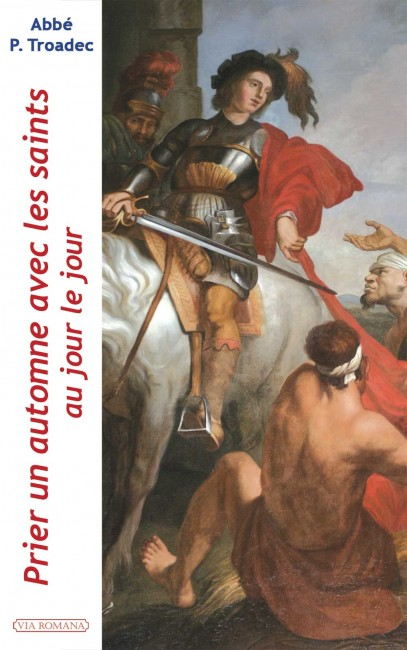
\includegraphics[angle=15,width=3cm]{img/prier-un-automne-avec-les-saints-au-jour-le-jour}
\end{wrapfigure}
\textbf{Retrouvez la vie de saint Front dans \emph{Prier un automne avec les saints} aux éditions \emph{Via Romana}. Disponible à la procure ou sur demande.}}
\end{document}
